\documentclass[english, 11pt]{article}
\usepackage{graphicx}
\usepackage{listings}
\usepackage{babel, blindtext, amsmath}
\usepackage[margin=0.8in]{geometry}
\usepackage{csquotes}
\title{Investigating $n^k$ $q$-player Tic-Tac-Toe winning strategies and their discoverability by machine learning algorithms.}
\author{David Kutner}
\begin{document}
\maketitle
\section*{Background}
Tic-Tac-Toe (known Noughts and Crosses in the UK), is a game ubiquitous in elementary schools and on the paper napkins of bored restaurant-goers. The game is played on a 3*3 grid, and two players take turns placing X's and O's, respectively, on empty cells, until one of the players controls three in a row (and that player wins) or no empty cells remain (and the game is a draw).
Formally and concisely, Tic-Tac-Toe is a two-player positional game; less concisely, we expound ``positional game" to mean:
\begin{description}
\item [Positional game:] a general category \textbf{zero-sum}, \textbf{perfect information} games in which players take turns placing symbols on a board of $P$ positions. There exist win-groups $WG \subseteq P$. If a player has filled a win-group $WG_i$ with her moves, then that player has won the game (in Tic-Tac-Toe, these correspond to the groups of positions that are along a straight line). If, on the other hand, the entire board is filled without either player gaining control of a full win-group, the game is called a draw \cite{krivelevick}.
\item [Zero-sum game:] a game in which any benefit for one subset of the players implies an equal loss across the complement of that subset. 
\item[Perfect-information game] all players have access to all of information about the current gamestate. Chess is another example of a perfect-information game. Poker is \textit{not} a perfect-information game.
\end{description}
Tic-Tac-Toe is the two-player positional game with $P = \{0,1,2,3,4,5,6,7,8\}$ and $WG = \{\{0,1,2\}, \{3,4,5\},\\ \{6,7,8\}, \{0,3,6\}, \{1,4,7\}, \{2,5,8\}, \{0,4,8\}, \{2,4,6\}\}$. 
%% include a figure numbering 0-8 on grid?

With 9 positions and the number of available positions reduced by one each turn, the total number of playable games (sequences of gamestates ending in a draw or win) is upper bounded by $9!=362880$. We call such a set of gamestates \textbf{naively enumerable}; a single-thread algorithm can rapidly process all possible gamestates in Tic-Tac-Toe without the use of either algorithmic shortcuts or high-level parallelization. In fact, the map of optimal moves can be concisely represented in a human-readable format which fits on half a page (see Fig. \ref{fig:xkcd}).
\begin{figure}[!h]
	\centering
	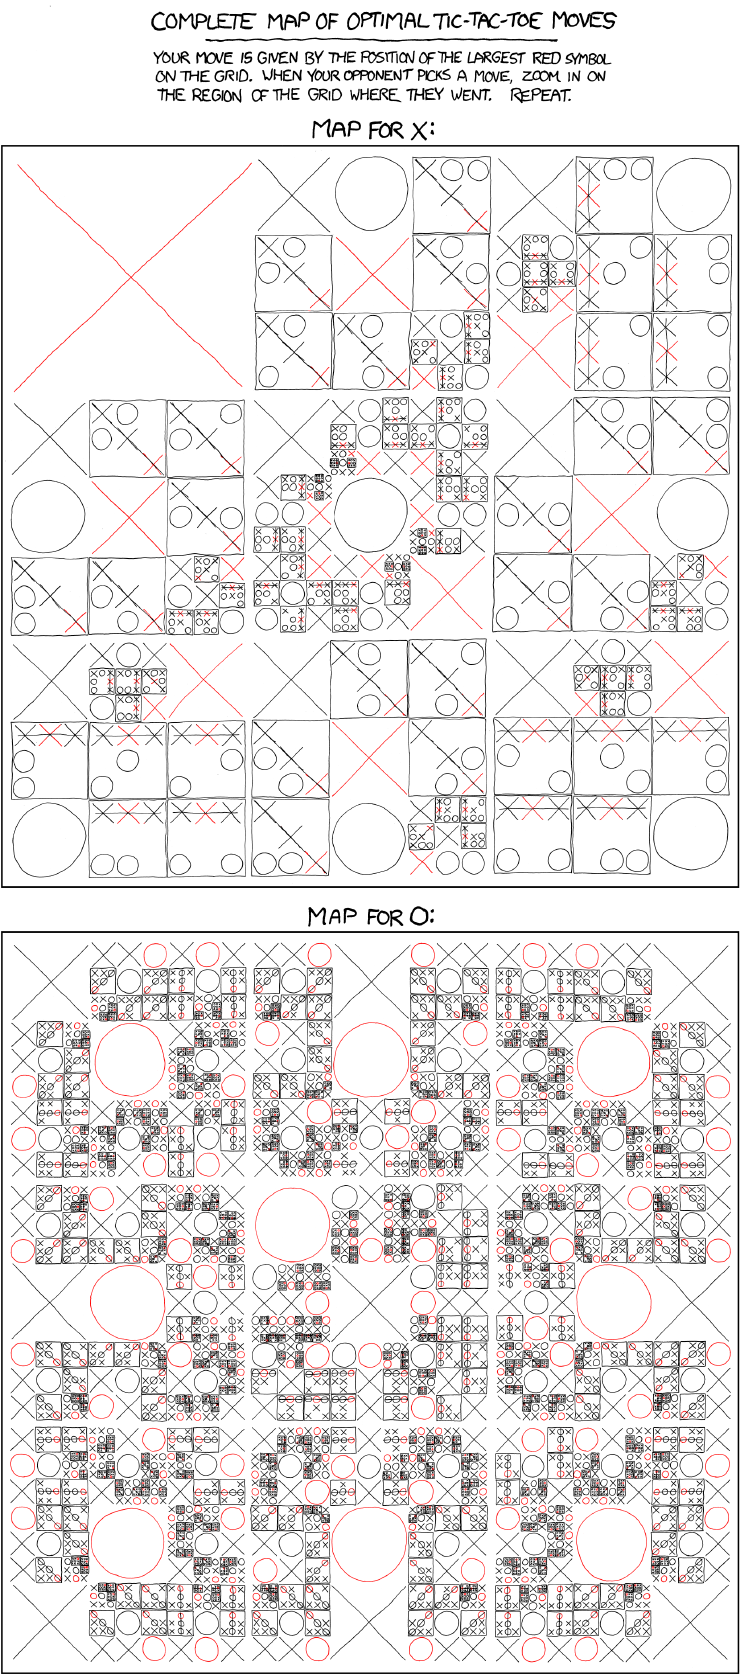
\includegraphics[scale=.2]{./img/xkcd.png}
	\caption{Map of optimal Tic-Tac-Toe moves \cite{xkcd}.} \label{fig:xkcd}
\end{figure}

\section*{Project background}

Hypercube ($n^k$) Tic-Tac-Toe is a game played on an $n*n*...*n$, $k$-dimensional ($n^k$) board, by 2 players. Each player takes turns placing an X or an O, respectively, on an empty cell on the board. The first player to “control” $n$ cells in a straight line wins \cite{golomb}. $3^2$ Hypercube Tic-Tac-Toe is exactly ``Classical" Tic-Tac-Toe, variations of which have existed for thousands of years \cite{marla}. Higher-dimension variants were conceived at least as early as 1955, when Qubic ($4^3$ Tic-Tac-Toe) was made commercially available \cite{55}.

In Qubic lines would now be depth- and width-wise rows, columns, any of the 4 diagonals between opposite corners, and any of the 24 diagonals in 2 dimensions.

Any game of Hypercube Tic-Tac-Toe necessarily belongs to \textbf{one of 5 categories} depending on the values of $n$ and $k$ \cite{golomb}:
\begin{displayquote}
	\begin{enumerate}
		\item The first player must win (as when $n=2$ for $k \geq 2$).
		\item Since no draw is possible, the first player should have a relatively easy win
		(as when $n = k = 3$, where playing in the center on the first move is already
		devastating).
		\item Although draws are possible, there is a win for the first player with best play.
		(It is known that exhaustive computer searching has shown that the $4^3$
		board is in this category.)
		\item Although there is no trivial drawing strategy for the second player (as in
		region 5, below), the second player can always draw with best play. (This is
		the case for the familiar $3^2$ board. While mathematicians will consider the
		drawing strategy “trivial” because it is so easily learned, it does not meet our
		definition of “trivial” given in Region 5; nor does it meet the layman's notion
		of “trivial” since this game is still widely played.)
		\item The second player has a “trivial” draw by a pairing strategy. In a pairing
		strategy, two of the $n^k$ cells are explicitly dedicated to each of the
		winning paths. (There may be some undedicated cells left over.)
		Whenever the first player claims one dedicated cell, the second player then
		immediately claims the other cell dedicated to the same path, if he hasn't
		already claimed it. (If he already has, he is free to claim any unclaimed cell.)
		Clearly, the first player can never complete a winning path if the second player
		is able to follow this strategy.
	\end{enumerate}
\end{displayquote}

For certain values of $n$, $k$, it is known which category the game belongs to;
Fig. \ref{fig:golomb_table} from Golomb's paper \cite{golomb} shows the categorization of games for given integers $n$ and $k$ as of 2002.

\begin{figure}[!h]
	\centering
	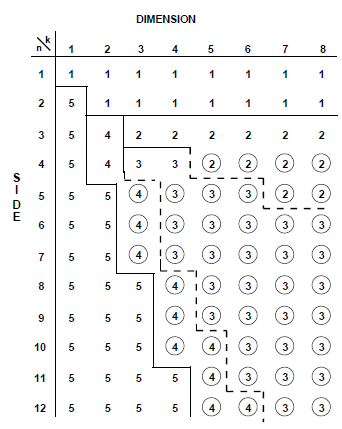
\includegraphics[scale=1]{./img/golomb.png}
	\caption{Regions (categories for games) in $n - k$ phase space. (Dotted boundaries and circled numbers
		are uncertain.) From Golomb's paper in 2002 \cite{golomb}.} \label{fig:golomb_table}
\end{figure}

Further, the below theorem implies that the union of categories 1 and 2 is infinite; if we take $c=2$ and the colors correspond to X and O respectively, then for each integer $n$ there exists at least one game ($n^k$ for some $k$) in which any ``full" board necessarily includes at least one winning path, i.e. it is impossible to draw.
Since only those games with $n\leq 2$ are in category 1 (in any game with $n \geq 3$ and $k \geq 2$, it is possible for the 2nd player to win), and \emph{all} those games with $k \leq 2, n \geq 2$ are in category 1, we have that both category 1 and category 2 are infinite. 
\begin{displayquote}
	\textbf{Theorem}: 
	For any positive integer values of n and c, there exists an integer k such that
	whenever the squares of the $n^k$ Tic-Tac-Toe board are colored in c colors, there exists a monochromatic winning path.\cite{mathellaneous}
\end{displayquote}

%%explain intuition behind Theorem?

Tic-Tac-Toe can also be extended in a different manner; one might increase the number $q$ of players. Patashnik points out that this quickly becomes computationally infeasible if we classify Tic-Tac-Toe as a $q$-player positional game and increase $q$ in that sense (each player gets their own symbol) \cite{patash}. We can, however, introduce more players without introducing more symbols to the board, as we describe below.

\section*{$q$-player $n^k$ Tic-Tac-Toe}


We then define our $q$-player $n^k$ Tic-Tac-Toe as the following game:

Each of $q$ players take turns placing X's and O's on empty cells of the hypercube board. The game ends when:
\begin{itemize}
\item The board has no more empty cells, in which case the game is a draw.
\item Any player controls all cells along a line, in which case that player wins and all other players lose. 
\end{itemize}

We choose to define this game as q players taking turns to place an O (on even-numbered moves) or an X (on odd-numbered moves) on the board. The first player to complete a line wins. An example of a 3-player, $3^2$ Tic-Tac-Toe game:
	\begin{enumerate}
		\item Player 0 places an X at (1,1)
		\item Player 1 places an O at (2,0)
		\item Player 2 places an X at (1,2)
		\item Player 0 places an O at (0,0)
		\item Player 1 places an X at (1,0) – player 1 wins, as their move completed the winning line {(1,1), (1,2), (1,0)}. 
	\end{enumerate}
	This game has the convenient property of preserving the equivalences which exist in 2-player $n^k$ Tic-Tac-Toe, for any value of $q$ (including 1), since the symbols on the board and condition for the game terminating remain the same; only the assignment of the win to a player, and therefore the players' decisions of where to place the symbols, change. A randomly played 8-player $7^8$ Tic-Tac-Toe game would be indistinguishable from a randomly played 3-player $7^8$ Tic-Tac-Toe game.

\textbf{Note:} we refer to a chosen $q$-player game played on some specified $n^k$ \textit{board} as a \textit{game}, and to each legal assignment of symbols to said board as a \textit{gamestate}.


\section*{Game categorizations}

Perhaps the most relevant property of a game with regard to how fun it would be to play is the existence or absence of a winning (or drawing) strategy. Plainly, a game in which one player can win regardless of the others' moves is not a fun game to play; conversely, a game in which it is impossible for \textit{any} player to win is uninteresting. The ideal game is one in which all players draw under perfect play, but mistakes on their opponents behalf open the possibility of a win for a player. 
We may therefore wish to outline what types of game divide the set of all Hyper-Tic-Tac-Toe games. For two players, those categories are outlined from Golomb above; for more than two players, however, these are not a set cover for all possible games. For instance, the $2^2$ game, when played with 3 or more players, is necessarily a win for the 3rd player (as with two players, the 3rd move \textit{must} win, regardless of player intention or ability).

\section*{Game tree}
The game tree for a game of Hyper-Tic-Tac-Toe is a rooted tree describing all possible outcomes of the game, in which the root is labeled with the empty board (starting gamestate), the leaves all correspond to terminal gamestates (wins and draws), and a node $c$ is another node $p$'s child iff $c$'s gamestate can be reached from $p$'s gamestate in exactly one move. Fig. \ref{fig:fulltree} shows the game tree for $2^2$, 2-player Tic-Tac-Toe. 
\begin{figure}[!h]
	\centering
	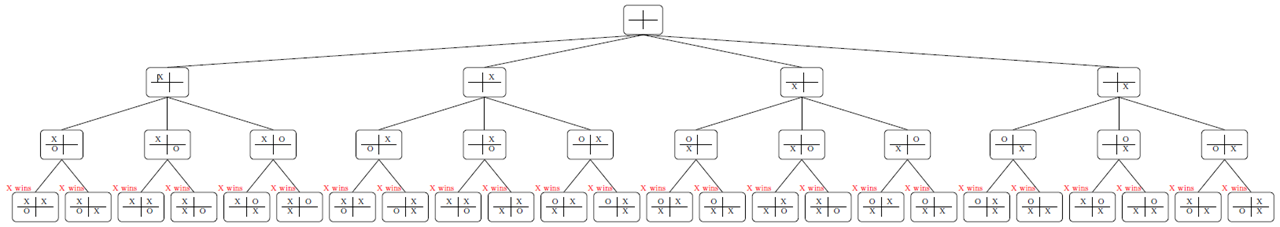
\includegraphics[scale=.65]{./img/fulltree.png}
	\caption{Game tree for $2^2$ Tic-Tac-Toe with 2 players.} \label{fig:fulltree}
\end{figure}
To prove that a winning strategy for player Q exists, we might construct the full game tree, then label leaves as Q-winnable as follows:
All those leaves whose gamestates are wins for Q are Q-winnable. 
Any node whose gamestate has Q next in the turn order is Q-winnable if \textbf{at least one} of its children is Q-winnable (the intuition being that player Q could choose to make that specific move rather than one which might allow their opponents to win).
Any node whose gamestate does \textit{not} have Q next in the turn order is Q-winnable if \textbf{all} of its children are Q-winnable (Q's opponents would likely identify and avoid branching into a Q-winnable gamestate). 
Thus, we can prove for any player Q through the generation of a full game tree whether the game is winnable by that player.
The same approach can be used to prove the existence of a drawing strategy; interestingly, there is a difference between proving that no player can force a win and proving that no player can force a draw - indeed, with more than 2 players, (say players X, O and Z), Z might in this situation block X's win (so the gamestate is not X-winnable, as X cannot count on Z to pass on this move) but might also allow X to win (the gamestate is therefore not O-drawable, since O cannot count on Z to block X).  

\section*{Oracle-guided game tree}
One might note that, if had an oracle to indicate the optimal moves for a player Q and we simply wished to verify that these moves did indeed constitute a winning strategy, we needn't build the entire game tree. Indeed, we may start from the root and:
\begin{itemize}
\item When it is Q's move, produce only the gamestate resulting from the oracle's move of choice.
\item For every other player's move, generate all possible children.
\end{itemize}
We then have a much smaller tree; indeed, where the full tree will have size $O(n^k!)$,  this Oracle-guided tree will have size $O((n^k!)^{\frac{q-1}{q}})$ (so for 2 players, the game tree would have size $O(\sqrt{n^k!})$).

\begin{figure}[!h]
	\centering
	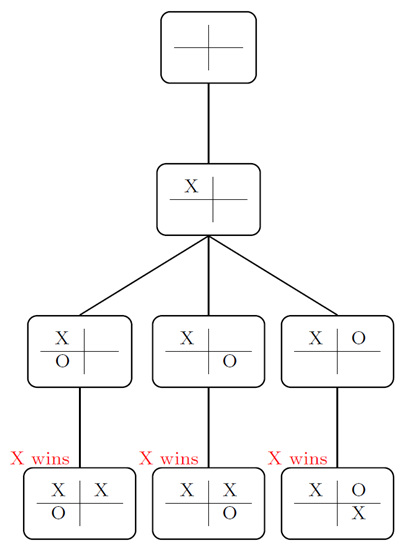
\includegraphics[scale=.65]{./img/isotree.png}
	\caption{Oracle-guided game tree for $2^2$ Tic-Tac-Toe with 2 players. (The oracle here is guiding X's moves).} \label{fig:isotree}
\end{figure}
If all leaves on the tree thus generated are wins for Q, then Q has a winning strategy. If all leaves on the tree thus generated are either wins for Q or draws, then Q has a drawing strategy, and might still have a winning strategy we haven't found (and our oracle is imperfect). If at least one of the leaves is a loss for Q, we learn nothing from this tree with regard to Q-winnability or -drawability of the game. 
In order to prove the game is impossible for Q to win, we would need to prove for every adversary A of Q's that a drawing-or-better strategy exists for A (though as explained in the section above \textbf{add diagram for example O X and Z above, refer to here}, even this doesn't exhaust all possibilities). 

\section*{Equivalent gamestates}

We can call two gamestates \textit{equivalent} if there exists a sequence of reflections and rotations mapping one gamestate onto another, as shown in Fig. \ref{fig:equivtree}. 

\begin{figure}[!h]
	\centering
	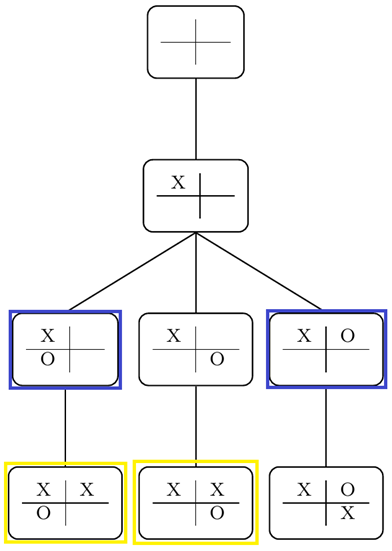
\includegraphics[scale=.65]{./img/equivtree.png}
	\caption{The oracle-guided game tree from Fig. \ref{fig:isotree} with equivalent gamestates highlighted.} \label{fig:equivtree}
\end{figure}

By removing equivalent gamestates when constructing our (oracle-guided) game trees, we can reduce the size of the tree we eventually produce significantly. By how much depends on the dimensionality ($k$) of the game board. If $k=1$ (the board is a series of cells in a straight line), for instance, then the only transformation is an inversion, and we will only reduce the tree's branching factor by a factor two at most. For $n$-dimension games, there exist $2^nn!$ transformations: a six-dimensional game board can be transformed in $2^6 6!=46080$ unique ways.

\section*{Choice of tools}

A basic operation (which we will refer to as ``gather") is implemented in plain python as follows:\\
\texttt{def gather(b, t):}\\
\indent \texttt{out = []}\\
\indent \texttt{for i in range(len(t)):}\\
\indent \indent \texttt{   out.append(b[t[i]])}
\indent \texttt{return out}\\

As we will see later in the report, this operation is the basic building block toward both the computation of equivalent gamestates (applying a transformation $t$ to a board $b$) and the computation of wins or losses ($t$ is the coordinates of points along a line and $b$ the board again). Therefore, it makes sense for us to experiment with different tools to implement the fastest-possible gather operation.
Several options were considered for the gather operation, which was implemented:
\begin{itemize}
\item In plain Python (as above) to serve as a benchmark for performance.
\item Using Numpy, which is implemented in C and frequently used to accelerate single-thread processing of data.
\item In plain C, which was compiled to a shared object and called from Python much as Numpy's functions are. The hope was that this would eliminate some of the overhead involved in Numpy's operations, getting us ``closer to the metal". 
\item Using PyTorch, which is optimized for operations on large tensors. Out of interest, the PyTorch experiments were carried out on the CPU as well as the GPU.
\item Using the Numba library for Python code precompilation, which is compatible with plain Python and Numpy. 
\end{itemize}
Fig. \ref{fig:unbatched} shows the time taken for a gather operation to be run on arrays of sizes between 9 and 128 (realistic board sizes for our work).
Although the best runtime is consistently that of precast C (in which the operation to obtain a pointer to the Numpy array's data was not included in the time taken), this implementation did not \textit{significantly} outperform the Numba-accelerated Numpy implementation. 
\begin{figure}[!h]
	\centering
	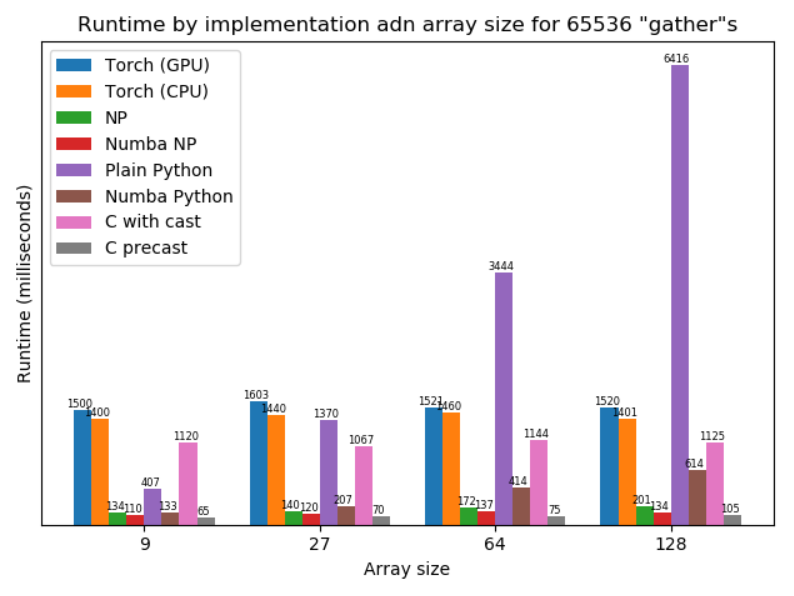
\includegraphics[scale=1]{./img/unbatched_full.png}
	\caption{The runtime for the gather operation, by array size and implementation. Note that Numba with Numpy performs nearly as well as precast C across all array sizes.} \label{fig:unbatched}
\end{figure}

Note that PyTorch in particular is underwhelming in its runtime, underperforming even plain Python for small array sizes. This is due to PyTorch being optimized for the quick computation of tensor (generally floating-point) operations taking up megabytes or gigabytes of space. Although there is little practical use (within the scope of our project) for the ability to compute whether a board of such a size is or is not a win, we can batch together many smaller boards (say of 64 cells each) to benefit from PyTorch's optimization. Fig \ref{fig:batched} shows just this.

\begin{figure}[!h]
	\centering
	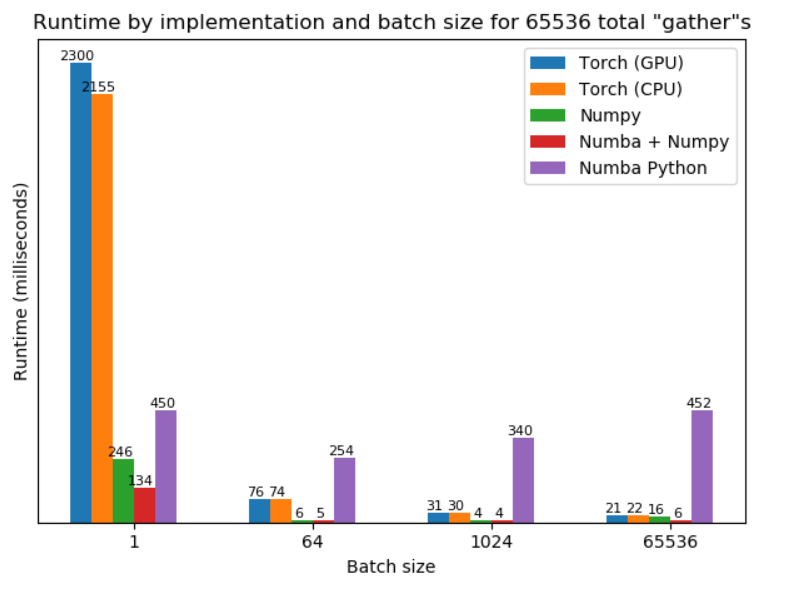
\includegraphics[scale=1]{./img/batched_full.png}
	\caption{The runtime for the gather operation, by batch size and implementation; the array size here was fixed at 64. Note to Tom: C implementations are absent because they would be a little more time-consuming to implement - I'll discuss this with you at our meeting.} \label{fig:batched}
\end{figure}

\pagebreak
\section*{Below - Unchanged sections from the Lit Survey, as explained in email}


\section{Definition of terms}

\begin{description}
	\item [Positional game:] a general category zero-sum (any benefit for one subset of the players implies an equal loss across the complement of that subset), perfect information (all players know the full state of the game when making their move) games in which players take turns placing symbols on a board of $P$ positions. There exist win-groups $WG \subseteq P$. If a player has filled a win-group $WG_i$ with her moves, then that player has won the game (in Tic-Tac-Toe, these correspond to the groups of positions that are along a straight line). If, on the other hand, the entire board is filled without either player gaining control of a full win-group, the game is called a draw \cite{krivelevick}.
	\item [Terminal configurations]: A configuration $C$ of $P$ is said to be terminal if and only if there are no empty positions or there exists a win-group that is completely occupied by a player. In the former case, the game is called a draw, and in the latter, the game is a win for whichever player just completed a win-group \cite{krivelevick}
	
	\item [$n^k$ Tic-Tac-Toe:] A semi-reasonable extension of Tic -Tac-Toe, played on a k-dimensional, n-wide board, created by bored mathematicians because things aren’t allowed to stay simple. 
	\begin{displayquote}
		 $n^d$ is a natural, yet extremely far reaching and challenging generalization of the classical Tic-Tac-Toe game. Given positive integers $d$ and $n$, the board $X$ of $n^d$ is the $d$-dimensional cube $X = [n]^d$, and the winning sets
		are the so-called \textit{geometric lines} in $X$. A geometric line $l$ is a family of $n$ distinct points
		$(a^{(1)}, a^{(2)}, . . . , a^{(n)})$ of $X$, where $a^(i) = (a_1^{(i)}, ..., a_d^{(i)})$ such that for each $1 \leq j \leq d$ the sequence of corresponding coordinates $(a_j^{(1)}, a_j^{(2)}, . . . , a_j^{(n)})$ is either $(1,2,...,n)$, or $(n, n-1, ..., 1)$ or constant (and of course at least one of the coordinates should be non-constant). The winner is the player who occupies a whole line first, otherwise the game ends in a draw. The familiar Tic-Tac-Toe is $3^2$ in this notation. \cite{krivelevick}
	\end{displayquote}
	\item [``Expert" moves:] those moves which do not guarantee perfect play, and are made by following a heuristic, applying machine learning, or are manually input by the researcher; referred to as ``strategic" moves in Patashnik's paper \cite{patash}.
	\item [``Brutish" moves:] moves which a computer player may find deterministically to guarantee perfect play (i.e. with a brute-force search of the branch of the game-tree resulting from the move). These moves are often \textbf{forced sequences}, which have a narrow (linear-size) game tree branch; referred to as ``tactical" moves in Patashnik's paper \cite{patash}.
	\item [Forced sequence: ] a sequence of moves from a given position in which player O must continually block player X’s $k$-in-a-row until at some move they must simultaneously block two such k-in-a-row’s, which is impossible, meaning player X wins \cite{patash}.
	\item [Categories 1-5:] 5 categories into which all $n^k$ Tic-Tac-Toe games fall, depending on whether and how they are winnable or drawable by player X or O, respectively. They are defined in the ``Project Background" section above.
	\item [$q$-player, $n^k$ Tic-Tac-Toe:] an abomination created by overzealous computer scientists so that they would have something to test out their shiny new machine learning algorithms on. 	
	We choose to define this game as q players taking turns to place an O (on even-numbered moves) or an X (on odd-numbered moves) on the board. The first player to complete a line wins. An example of a 3-player, $3^2$ Tic-Tac-Toe game:
	\begin{enumerate}
		\item Player 0 places an X at (1,1)
		\item Player 1 places an O at (2,0)
		\item Player 2 places an X at (1,2)
		\item Player 0 places an O at (0,0)
		\item Player 1 places an X at (1,0) – player 1 wins, as their move completed the winning line {(1,1), (1,2), (1,0)}. 
	\end{enumerate}
	This game has the convenient property of preserving the equivalences which exist in 2-player $n^k$ Tic-Tac-Toe, for any value of $q$ (including 1), since the symbols on the board and condition for the game terminating remain the same; only the decision of where to place the symbols changes. A randomly played 8-player $7^8$ Tic-Tac-Toe game would be indistinguishable from a randomly played 3-player $7^8$ Tic-Tac-Toe game.
	\item [Game tree:] a tree corresponding to all possible games for given integers $n$  and $k$. In this tree:
	\begin{itemize}
		\item every node $q_i$ corresponds to a configuration $c_j$. It is possible that some other nodes also correspond to the same configuration(this is the case when the same set of moves is played in a different order). 
		\item nodes are divided into $q$ sets $Q_0, ..., Q_{q-1}$ corresponding to the q players. The child of a node in $Q_i$ is in $Q_{i+1\mod q}$.
		\item the root node $q_0$ corresponds to the empty board $c_0$, and is in $Q_{q-1}$ since the next move will be made by player 0 (and so is in $Q_0$). 
		\item a node is a leaf (has no children) if its configuration is a terminal one (as in the definition above). 
		\item the children of a node $q_i$ with board $c_j$ correspond to those boards reachable from $c_j$ in one move (which must be an X- or O- move if the node $q_i$ is in the set X or the set O, respectively). These configurations are said to be the \textbf{successors} of $c_j$. 
	\end{itemize}  
	\item [Equivalent configurations: ] two configurations $C_1$ and $C_2$ are said to be \emph{equivalent} if there exists a ``one-to-one mapping of the set of points onto itself that preserves the set of lines" \cite{patash}. In these cases, one of the two positions is \textbf{redundant}. One example would be where $C_2$ is the reflection or rotation of $C_1$. 
\end{description}

\section{Program efficiency and parallelism}

In 1980, Oren Patashnik proved that $4^3$ Tic-Tac-Toe (Qubic) is a first-player-win with optimal play on both players’ sides. This required the use more than 1500 hours of CPU time; he estimated that half of these were wasted (were the result of backtracking after a faulty manually input move), and that he could have optimized his program by implementing it in a “lower level language instead of Algol” to reduce the time taken to solve the problem by ``more than an order of magnitude", which leaves us at an estimate of 75 hours of CPU time to prove that Qubic does indeed belong to region 3. Patashnik manually input nearly 3000 first-player moves himself \cite{patash}. 

If we are to match (and ideally outperform) Patashnik’s program runtime without relying on a (very tired) programmer to manually input intuitive, optimal moves, we need to:
\begin{enumerate}
	\item Prune the search tree by identifying equivalent configurations.
	\item Make use of parallelism both at each individual node and to run the entire search.
	\item Substitute Machine Learning in the place of human intuition.
\end{enumerate}

\subsection{Pruning the search tree}
In order to reduce search time, at each step of a “naïve” breadth-first- search (which allows us to with all boards having seen m moves at one time) we identify and terminate search nodes whose configurations are redundant (equivalent to another non-terminated node’s configuration)\cite{patash}. 
Although it is possible for two boards in a general game to be isomorphic (equivalent) without having the same number of moves \cite{antoy}, the memory and performance constraints imposed by having to process pairs of boards across all different levels of the search tree mean that the task is computationally not worthwhile – $O((b^d)^2)$, with b the branching factor once same-level pruning has been applied and d the depth - even if it were fast to carry out for any individual pair, which it isn’t. 
\subsection{Parallelism}
From our definition of  $n^k$ Tic-Tac-Toe above \cite{krivelevick}, we notice that to check whether a game constitutes a win involves many vector operations on the k-vectors describing the moves of each player. Such operations can be optimized through parallel programming \cite{bsp}; as a matter of fact, these operations are precisely those which modern GPUs are designed to carry out in bulk, swiftly \cite{cuda}. 
One might therefore seek to implement a function which determines whether a given board (tuple $(n, k, O, X)$ is a terminal board (that is, either is full or one of the sets $O$ and $X$ contain a winning set of moves) using as much matrix- and vector- arithmetic as possible, to enable the operations to be carried out swiftly, in parallel.
The use of parallelism also extends to growing the search tree; one might use a lock-based method to protect shared date between threads, although this “suffers from synchronization overhead due to thread contentions” \cite{montecarlo}. Mirsoleimani’s paper discusses the parallelization of operation-level tasks (as opposed to iteration-level tasks) in a Monte-Carlo tree search, an optimization which appears to be generalizable to a “generic” breadth-first-search.
\subsection{Machine learning}
Machine Learning has begun to outperform humans at making “expert” moves \cite{NYT_Go}. It follows, then, that Machine Learning may be the answer to our problem with Patashnik’s approach; in our case, the researcher lacks the ability to manually input 3000 good moves into the program to prove the existence of a first-player-win, and specifically lacks the ability to reason in $k$ dimensions; if we would like an agent which is generalizable to $k$ dimensions, we may turn to Machine Learning to provide us with (approximations of) perfect moves. 
Deep learning is “designed for massive data sets with many high dimensional input variables”, which may involve up to “~1-2 billion parameters”. The Python library Tensorflow grants us both ease of implementation and access to a “state-of-the-art framework for a plethora of [Machine Learning] architectures” \cite{sokolov_polson}. 


\section{The Project}

The project’s objectives is to expand Golomb’s table into the third dimension, where $q$ is increased from its traditional value of 2, and to find trends in how these regions grow in the 3rd dimension, allowing us to conjecture (and possibly prove) the categorization of certain games as a function of n, k, and q. 
A fast win-check function as well as an equivalent (redundant) board identifier will be implemented in C (chosen for being low-level and -somewhat- easily ported into Python) and integrated into the main program if the runtime of this implementation compares favorably to a Python implementation using Numpy or other matrix- and tensor- operation packages. This function will be compiled and made callable in Python, to enable the use of the PyTorch package. 
A reinforcement learning algorithm will be implemented in PyTorch. It should, with enough training: 
\begin{enumerate}
	\item Never, as either player, lose a game which is in category 4 (where a “trivial” drawing strategy exists for player O).
	\item Always, as player X, win games in categories 1 or 2 (where draws are impossible – i.e. never lose a game in these regions).
	\item Always, as player X, win game in category 3 (where draws are possible, but a winning strategy is known to exist for the first player).
	\item Against random play, win with high probability those games in region 4 (where non-trivial drawing strategies exist) as well as those games whose region is uncertain and may be 4 (i.e. large values $n$ and $k$, e.g. $n=12, k=5$), as either player. 
	
\end{enumerate}

This algorithm will be generalizable to the q-player game, and will serve to provide the “expert” moves in proving which region each game (corresponding to some positive integers $q, n, k$) belongs to in n-k-q space. This should reduce search tree size – for instance $T$ originally – to $T^\frac{q-1}{q}$:
Suppose we have an expert player, and that we wish to prove that the $q$-player $n^k$ game of Tic-Tac-Toe is always winnable (drawable) by player $i$ with perfect play. We build the partial game tree as follows:
\begin{itemize}
	\item Start at the root node $q_0$. 
	\item At each node which is not in the set $Q_i$, produce all possible successors from the corresponding configuration (and eliminate duplicates).
	\item At each node which \emph{is} in the set $Q_i$, only produce a single successor, which is provided by the expert. 
\end{itemize}
If every leaf in the guided game tree is a win (draw) for Player $i$, then we have proven that there exists a winning (drawing) strategy for that player, since every possible move for the other players was considered. On the other hand, if this is not the case, we have not proven anything, since we cannot guarantee that our ``expert" algorithm is playing optimally. 
To prove that Player $i$ always \emph{loses} with perfect play, we must carry out the above for every player other than Player $i$ and show that these players always win under perfect play (which implies a loss for $i$). 
An advanced objective of this project would be to prove the region membership of one of the “uncertain” games in Golomb’s paper (with $q=2$). 


\begin{thebibliography}{99}
	\bibitem{marla} Parker, Marla \textit{ She Does Math!: Real-life Problems from Women on the Job.} (1995). Mathematical Association of America. p. 153. ISBN 978-0-88385-702-1.

	\bibitem{xkcd}	
	Munroe, Randall \textit{XKCD 832: Tic-Tac-Toe}. (2010) Retrieved from https://xkcd.com/832/. 
	
	\bibitem{golomb}	
	Golomb, Solomon W., Hales, Alfred W. \textit{Hypercube tic-tac-toe}. \textit{More Games of No Chance }. (2002) Math. Sci. Res. Inst. Publ. Cambridge Univ. Press. 42: 167–182. MR 1973012.
	
	\bibitem{55}
	\textit{Three-Dimensional Tic-Tac-Toe Game}. Journal of the Franlin Institute 1955, Vol.259(1), pp.85-85.
	
	\bibitem{mathellaneous} 
	Do, Norman. \textit{Mathellaneous}. University of Melbourne. Retrieved from http://users.monash.edu/~normd/documents/Mathellaneous-01.pdf.
	
	
	\bibitem{patash}
	Patashnik, Oren. \textit{Qubic: $4*4*4$ Tic-Tac-Toe}, \textit{Mathematics Magazine} Vol. 53, No. 4 (September 1980) pp. 202-216. 
	
	\bibitem{NYT_Go}
	Mozur, Paul. \textit{Google’s AlphaGo Defeats Chinese Go Master in Win for A.I.}, \textit{The New York Times} (March 2017), retrieved from https://www.nytimes.com/2017/05/23/business/google-deepmind-alphago-go-champion-defeat.html. 
		
	\bibitem{antoy}
	Antoy, Sergio. \textit{Modelling and Isomorphisms of Positional Board Games}.\textit{ IEEE Transactions on pattern analysis and machine intelligence} (1987).
	
	\bibitem{sokolov_polson}
	Polson, Nicholas G. and Sokolov, Vadim. \textit{Deep Learning: A Bayesian Perspective}. \textit{Bayesian Analysis} (2017).
	
	\bibitem{krivelevick}
	Krivelevich, Michael. \textit{Positional Games} (2014).
	
	\bibitem{bsp} 
	Yzelman, A. ; Bisseling, R. ; Roose, D. ; Meerbergen, K. \textit{Multicore BSP for C: A High-Performance Library for Shared-Memory Parallel Programming}. \textit{International Journal of Parallel Programming} (2014).
	
	\bibitem{montecarlo} 
	Mirsoleimani, S. Ali ; Plaat, Aske ; Herik, Jaap Van Den ; Vermaseren, Jos. \textit{Structured Parallel Programming for Monte Carlo Tree Search} (2017).
	
	\bibitem{cuda}
	Sanders, J. ; Kandrot, E. \textit{CUDA by example: an introduction to general-purpose GPU programming}. NVIDIA Corporation, 2010.
	
	\bibitem{hyperoctahedral} Hyperoctahedral Group. (n.d.). In Wikipedia. Retrieved April 13, 2020, from https://en.wikipedia.org/wiki/Hyperoctahedral\_group
\end{thebibliography}

\end{document}